% Force arXiv to process with pdflatex.
\pdfoutput=1

% Support alternating row colours in tables. Normal usage is to
% include the xcolor package with option `table', but the xcolor
% package is already getting pulled in from somewhere else which
% causes builds to fail with a package options conflict.
%
% See: http://tex.stackexchange.com/a/5375
%
\PassOptionsToPackage{table}{xcolor}

\documentclass{article}

\usepackage{arxiv}
\usepackage[utf8]{inputenc} % allow utf-8 input
\usepackage[T1]{fontenc}    % use 8-bit T1 fonts

\rhead{\textsc{ProGraML}: Graph-based Deep Learning for Program Optimization and Analysis}

% Maths.
\usepackage{bm}
\usepackage{amsfonts}
\usepackage{amsmath}

% Tables.
\usepackage{booktabs}
\usepackage{tabularx}
\usepackage{hhline}
\usepackage{xspace}
\usepackage[table]{xcolor}
\usepackage{multirow}
\usepackage{subcaption}
% Define column types L, C, R with known text justification and fixed widths:
\usepackage{array}
\newcolumntype{L}[1]{>{\raggedright\let\newline\\\arraybackslash\hspace{0pt}}m{#1}}
\newcolumntype{C}[1]{>{\centering\let\newline\\\arraybackslash\hspace{0pt}}m{#1}}
\newcolumntype{R}[1]{>{\raggedleft\let\newline\\\arraybackslash\hspace{0pt}}m{#1}}

% \usepackage{subfig}

% Reset footnote counter on every page.
\usepackage{perpage}
\MakePerPage{footnote}

% Add \cmark and \xmark for check and cross symbols, respectively.
\usepackage{amssymb}
\usepackage{pifont}
\newcommand{\cmark}{\ding{51}}%
\newcommand{\xmark}{\ding{55}}%
% Images
\usepackage{graphicx}

\newcommand\todo[2]{\textcolor{red}{\footnotesize \emph{TODO(#1): #2}}}
\newcommand{\bigo}{\mathcal{O}}
\newcommand{\ourproject}{ML4PL}

\usepackage{dsfont}

\title{ProGraML: Graph-based Deep Learning for\\Program Optimization and Analysis}

\author{%
  Chris Cummins\thanks{Both authors contributed equally}\\
  School of Informatics \\
  University of Edinburgh \\
  \texttt{c.cummins@ed.ac.uk} \\
  \And
  Zacharias V. Fisches\textsuperscript{*}\\
  Department of Computer Science \\
  ETH Zurich \\
  \texttt{zfisches@student.ethz.ch} \\
  \And
  Tal Ben-Nun \\
  Department of Computer Science \\
  ETH Zurich \\
  \texttt{talbn@inf.ethz.ch} \\
  \And
  Torsten Hoefler \\
  Department of Computer Science \\
  ETH Zurich \\
  \texttt{htor@inf.ethz.ch} \\
  \And
  Hugh Leather \\
  School of Informatics \\
  University of Edinburgh \\
  \texttt{hleather@inf.ed.ac.uk} \\
}

\begin{document}

\maketitle
\begin{abstract}
Machine learning (ML) is increasingly seen as a viable approach for building
compiler optimization heuristics, but many ML methods cannot replicate even the
simplest of the data flow analyses that are critical to making good optimization
decisions. We posit that if ML cannot do that, then it is insufficiently able to
reason about programs. We formulate data flow analyses as supervised learning
tasks and introduce a large open dataset of programs and their corresponding
labels from several analyses. We use this dataset to benchmark ML methods and
show that they struggle on these fundamental program reasoning tasks. We propose
\programl{} -- \emph{Program Graphs for Machine Learning} -- a
language-independent, portable representation of program semantics. \programl
overcomes the limitations of prior works and yields improved performance on
downstream optimization tasks.

\end{abstract}


\section{Introduction}

Compiler implementation is a complex and expensive activity~\citep{Cooper2012}.
For this reason, there has been significant interest in using machine learning
to automate various compiler tasks~\citep{Allamanis2017a}. Most works have
restricted their attention to selecting compiler heuristics or making
optimization decisions~\citep{leather2020mlinc}. Whether learned or engineered
by human experts, these decisions naturally require reasoning about the program
and its behavior. Human experts most often rely upon \textit{data flow}
analyses~\citep{Kildall1973,Kam1976}. These are algorithms on abstract
interpretations of the program, propagating information of interest through the
program's control-flow graph until a fixed point is reached~\citep{Kam1977}. Two
examples out of many data flow analyses are: \emph{liveness} -- determining when
resources become dead (unused) and may be reclaimed; and \emph{available
expressions} -- discovering which expressions have been computed on all paths to
points in the program. Prior machine learning works, on the other hand, have
typically represented the entirety of the program's behavior as a fixed-length,
statically computed feature vector~\citep{Ashouri2018}. Typical feature values
might be the number of instructions in a loop or the dependency depth. The
demonstrable weakness of these techniques is that they are trivially confused by
the addition of dead code, which changes their feature vectors without changing
the program's behavior or its response to optimizations. Such learning
algorithms are unable to learn their own abstract interpretations of the program
and so cannot avoid these pitfalls or more subtle versions
thereof~\citep{Barchi2019a}.

\begin{figure}[t]
 \centering %
 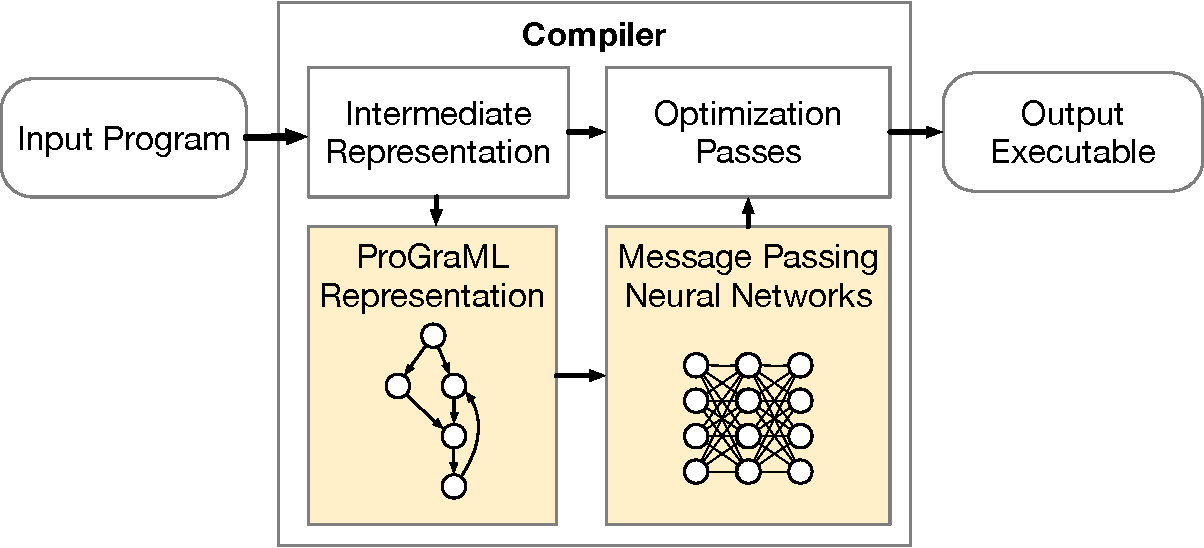
\includegraphics[width=.85\linewidth]{images/overview}
 \caption{%
    Our proposed approach for compiler analyses driven by graph-based deep
    learning.%
 }%
 \label{figure:overview}%
\end{figure}

Recently, there have been attempts to develop representations that allow
finer-grain program reasoning. Many, however, are limited both by how inputs are
represented as well as how inputs are processed. Representations based on source
code and its direct artifacts (e.g.,
AST)~\citep{Alon2018a,Yin2018,Haj-Ali2019,cummins2017synthesizing} put
unnecessary emphasis on naming and stylistic choices that may not correlate with
the functionality of the code (e.g., Fig.~\ref{subfig:code2vec}). Approaches
based on intermediate representations
(IR)~\citep{Ben-nun2018,Mirhoseini2017,Brauckmann2020} remove such noise but
fail to capture information about the program that is important for analysis
(e.g.,  Fig.~\ref{subfig:cdfg} variables, Fig.~\ref{subfig:inst2vec}
commutativity). In both cases, models are expected to reason about the flow of
information in programs using representations that do not directly encode this
information. Clearly, a program representation is needed that enables machine
learning algorithms to reason about the execution of a program by developing its
own data flow analyses.

Since current approaches are ill-suited to program-wide data flow analysis, we
propose overcoming some of their limitations by making the program's control,
data, and call dependencies a central part of the program's representation
\emph{and} a primary consideration when processing it. We achieve this by seeing
the program as a graph in which individual statements are connected to other
statements through relational dependencies. Each statement in the program is
understood only in the context of the statements interacting with it. Through
relational reasoning~\citep{Battaglia2018}, a latent representation of each
statement is learned that is a function of not just the statement itself, but
also of the (latent) representations of its graph neighborhood. Notably, this
formulation has a striking similarity to the IRs used by compilers, and the
iterative propagation of information resembles the \emph{transfer functions} and
\emph{meet operators} in traditional data flow analyses~\citep{Kildall1973}.

Recently proposed techniques for learning over graphs have shown promise in a
number of domains~\citep{Li2018a}. With a suitable representation and
graph-based model, we extend these approaches to the domain of compiler
analysis, enabling downstream tasks built on top of such graph models to
natively incorporate reasoning about data flow into their decision making. This
improves performance on downstream tasks without requiring additional features,
although challenges with respect to generalization to large programs at
test-time remain and are discussed in detail. Figure~\ref{figure:overview}
illustrates our approach. We make the following contributions:

\begin{itemize}
\item
We propose a portable, language-independent graph representation of programs
derived from compiler IRs.
\programl\footnote{\url{https://github.com/ChrisCummins/ProGraML}}
simultaneously captures whole-program control-, data-, and call relations
between instructions and operands as well as their order and data types.
\programl is a compiler-agnostic design for use at all points in the
optimization pipeline; we provide implementations for LLVM and XLA IRs.
\item
We introduce a benchmark dataset that poses a suite of established compiler
analysis tasks as supervised machine learning problems.
\textsc{DeepDataFlow}~\cite{chris_cummins_2020_4247595} comprises five tasks
that require, in combination, the ability to model: control- and data-flow,
function boundaries, instruction types, and the type and order of operands over
complex programs. \textsc{DeepDataFlow} is constructed from 461k real-world
program IRs covering a diverse range of domains and source languages, totaling
8.5 billion data flow analysis classification labels.
\item
We adapt Gated-Graph Neural Networks (GGNN) to the \programl representation. We
show that, within a bounded problem size, our approach achieves $\ge 0.939$
F$_1$ score on all analysis tasks, a significant improvement over
state-of-the-art representations. We set a new state-of-the-art on two
downstream optimization tasks for which data flow analyses are important.
\end{itemize}

\section{Motivation}

Machine learning promises significant benefits for simplifying and
improving the construction of optimization heuristics by replacing
fragile and expensive hand-tuned heuristics with data-driven
statistical modeling. For this goal to be realized, we require machine
learning systems capable of reasoning about program semantics. Despite
tremendous gains in recent years, state-of-the-art approaches for
learning on code are not sufficiently powerful to replicate the
analysis tasks that are fundamental to compilers. The crux of the
problem lies in two central aspects of machine learning: input
representation and model algorithmic complexity.

\paragraph{(I) Input Representation}

To be processed by a Neural Network (NN), code inputs may be encoded
either directly from a source language, by way of AST analysis, or
using an IR. Examples of each abound in the
literature~\cite{Allamanis2017a,Chen2019,Wang2018}. One
state-of-the-art encoder, code2vec~\cite{Alon2018a}, uses AST paths to
embed programs. code2vec proves highly effective at software
engineering tasks such as algorithm classification, where the code was
written by humans. However, as shown in Figure \ref{subfig:code2vec},
the trained representation can put more weight on names rather than
code structure, where minute modifications completely change
classification outcome. There are many benefits to such a
representation, including smart pasting and automated
refactoring. However, when analyzing code for optimization, identifier
names are rarely of use, whereas structure and semantics should be the
primary consideration. For example, in choosing to represent code at
the AST level, the code2vec representation does not capture the data
or control relations between statements.

\begin{figure}[t]
  \centering
    \begin{subfigure}{.48\linewidth}
      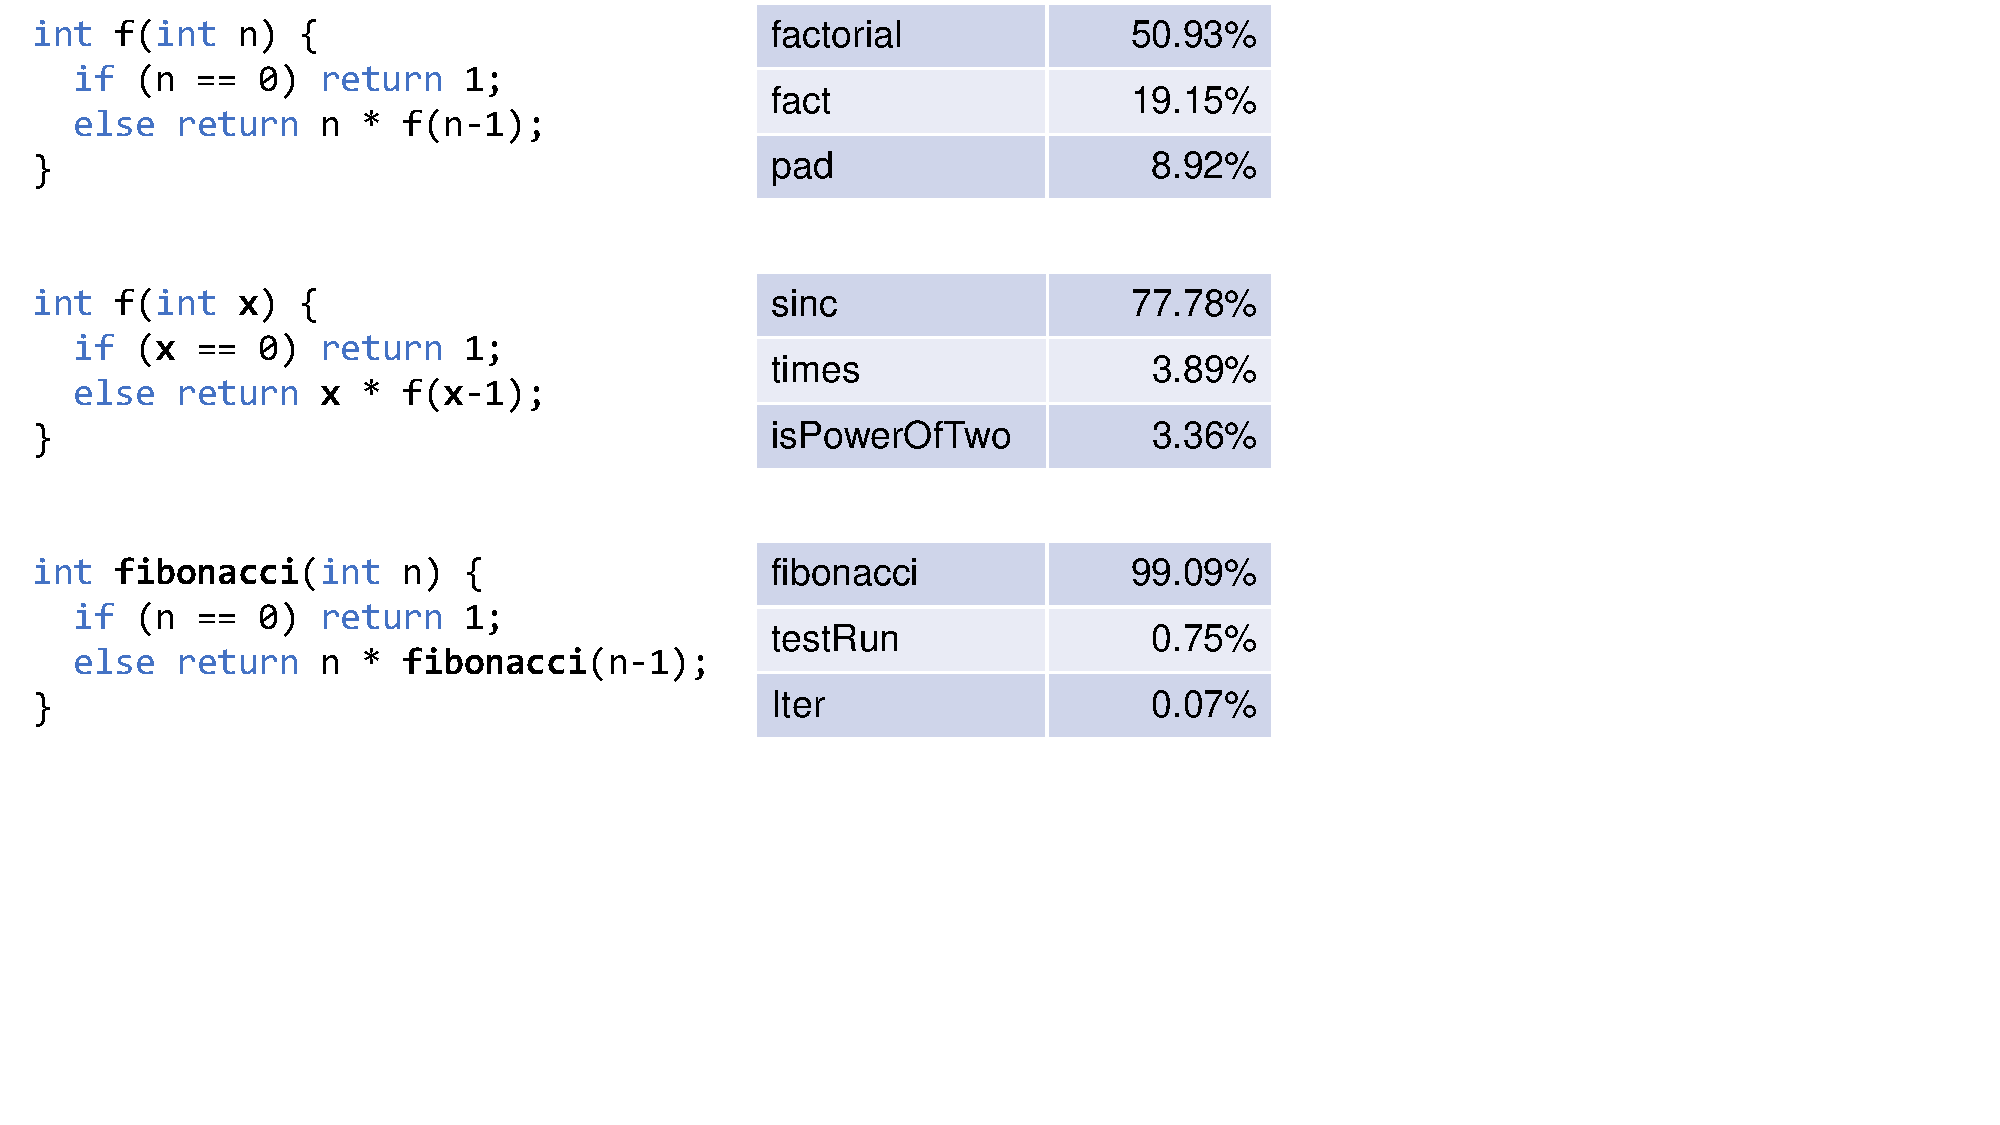
\includegraphics[width=\linewidth]{images/code2vec-transposed.pdf}
      \caption{code2vec~\cite{Alon2018a}.}
      \label{subfig:code2vec}
  \end{subfigure}
  \hfill
  \begin{subfigure}{.29\linewidth}
    \vspace{2.5em}
      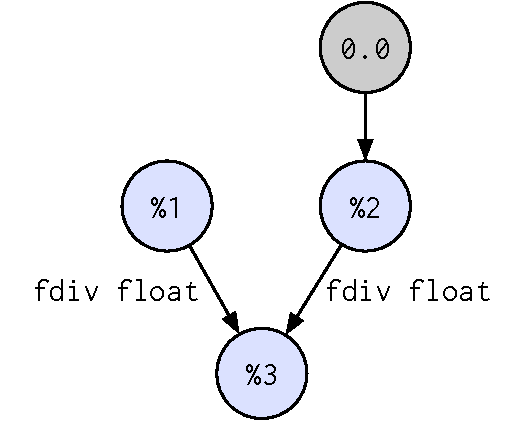
\includegraphics[width=\linewidth]{images/inst2vec.pdf}
      \caption{XFG~\cite{Ben-nun2018}.}
      \label{subfig:inst2vec}
  \end{subfigure}
  \hfill
  \begin{subfigure}{.18\linewidth}
  \vspace{2.4em}
  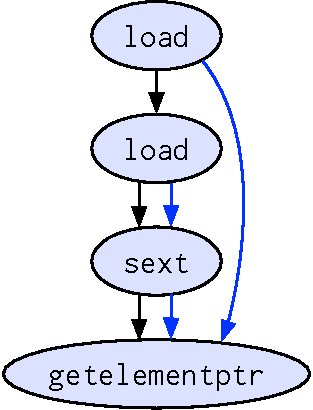
\includegraphics[width=\linewidth]{images/cdfg.pdf}
  \caption{CDFG~\cite{Brauckmann2020}.}
  \label{subfig:cdfg}
  \end{subfigure}
  \caption{%
    Limitations in state-of-the-art learnable code
    representations. In~(\subref{subfig:code2vec}) the model
    over-emphasizes identifier names such that the same algorithm
    produces three different classifications by changing the name of a
    function. The data-flow representation
    of~(\subref{subfig:inst2vec}) does not capture operand order, such
    that non-commutative statements such as division are
    indistinguishable. In~(\subref{subfig:cdfg}) control and data
    relations are captured, but both type information and operand
    order are omitted. Our approach is insensitive to identifier names
    and preserves operand order and type information.%
  }%
\end{figure}


An alternate approach which emphasizes semantics is Neural Code
Comprehension~\cite{Ben-nun2018}, where an encoder uses Contextual
Flow Graphs (XFG) built from LLVM-IR statements to create inputs for
neural networks. The XFG combines partial data- and control-flow to
represent the context of an individual statement. The statements are
then mapped to latent-space representations using their neighbors in
that graph. However, in partially combining DFGs and CFGs, the XFG
representation omits important information such as order of
instruction operands (as shown in Figure~\ref{subfig:inst2vec}), and
the representation fails to capture execution order, critical for many
optimization tasks.

A recent LLVM-IR representation uses Control and Data Flow Graphs
(CDFG)~\cite{Brauckmann2020}. This representation makes the control
and data relations between instructions explicit, but uses only
instruction opcodes to compute latent representations. This omits
information about programs that may be critical for optimization, such
as data types, the presence of variables and constants, and the
ordering of operands, shown in Figure~\ref{subfig:cdfg}.

Each of the three methods of encoding programs as inputs to neural
networks omit information that is vital for compiler analysis. This
hinders the ability of machine learning models to reason about
optimizations and their impact on program behavior. To address these
shortcomings we require an input representation that captures all
parts of a program's semantics that are required for performing such
analyses.


\paragraph{(II) Model Complexity}

The range of core operators in deep learning on code is largely
confined to recurrent units (e.g. RNN, LSTM, GRU) on sequences. This
poses limitations on the representation space of any such network's
outputs. Take, for instance, dominator tree construction. An LSTM
iterating forward over input code will not be able to solve the task
\emph{by definition}, as statements needs to be analyzed backwards
with respect to dependencies. Yet, the neural network only maintains
$\bigo(1)$ memory capacity w.r.t. program length. Iterating in the
opposite direction, in addition to being problem-specialized, would
still not suffice, as dependencies may ``vanish'' in the corresponding
gradients if dependent statements are far away from each other, such
as in the presence of diverging control flow.

One way to increase the algorithmic complexity of the model is by
allowing it to increase the number of code tokens that are processed
simultaneously during inference. This approach, commonly used in
literature by Transformer Networks~\cite{Vaswani2017}, use preceding
tokens (unidirectional encoding) or preceding and subsequent tokens
(bidirectional encoding) to learn \textit{attention matrices}. Such
matrices ``focus'' the network on certain subsets of tokens, skipping
others. However, this approach scales quadratically in memory and
computation with the number of tokens.

Unlike in natural language text, the dependency structure of code is
made explicit during compilation. We can thus employ domain-specific
knowledge to construct the attention matrices in a scalable manner,
using a graph representation of the tokens with dependencies as
edges. A graph representation not only enables meaningful attention
learning, but also facilitates propagating information across the
graph in a manner similar to typical compiler analyses. Within the
same step, a recurrent unit generates $\bigo(1)$ activations, whereas
a graph NN generates $\bigo(|V|)$.

To demonstrate this expressive power, let us consider control-flow
reachability analysis as a learning task. The goal of the model is to
tag statements that are reachable from one or more given tagged
statements. With a sequential LSTM, the model would have to be trained
to memorize nodes along some linear order of the given program. With
an unbounded number of nodes to track and variably-sized regions to
skip, the task becomes infeasible. A message-passing graph neural
network, in contrast, needs only to learn to pass a message forward in
the case of an existing control-flow edge between two nodes,
essentially learning an identity operation over control-flow edges and
zero on others.

In this work, we overcome the above limitations of prior model and
representation approaches, leveraging the graph structure of IR code,
taking path analysis and the semantics of individual statements into
account.

\section{A Graphical Program Representation for Analysis and Optimization}
\label{sec:graph-representation}

For machine learning to successfully reason over programs, a suitable
input representation must be used. This section presents
\textsc{ProGraML}, a novel program representation that closely matches
the representations used traditionally within compilers and can be
processed natively by machine learning models. Unlike prior approaches
that rely on hand-engineered feature
extractors~\cite{Ashouri2018,Wang2018} or which are closely tied to
the syntax of the target program language~\cite{Allamanis2017b}, our
approach captures whole-program control, data, and call relations and
is both task- and language-agnostic.

\begin{figure*}
  \centering %
  \begin{subfigure}{.48\linewidth}%
    \centering
    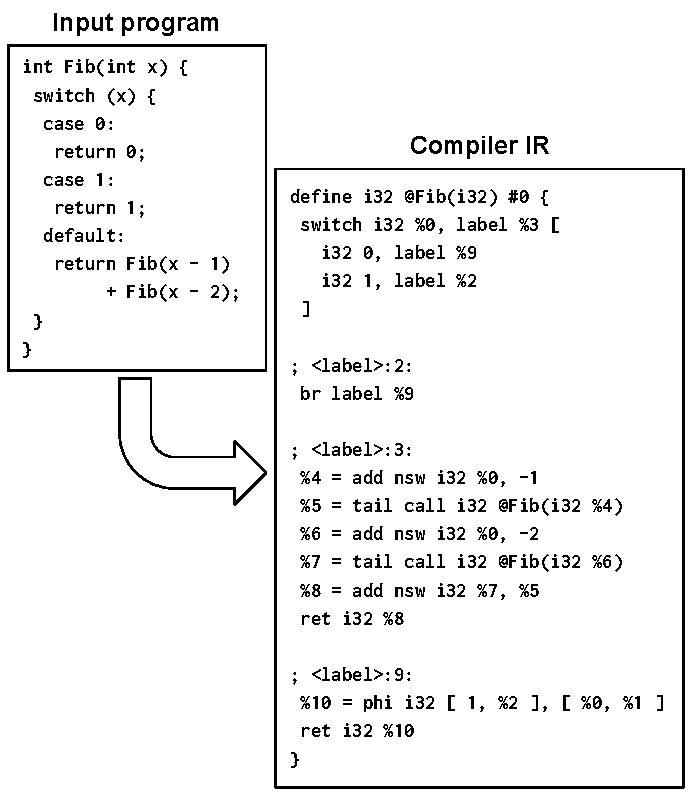
\includegraphics[width=\linewidth]{images/A_IR}%
    \caption{Compiler intermediate representation.}
    \label{subfigure:ir}%
  \end{subfigure}
  \begin{subfigure}{.48\linewidth}%
    \centering
    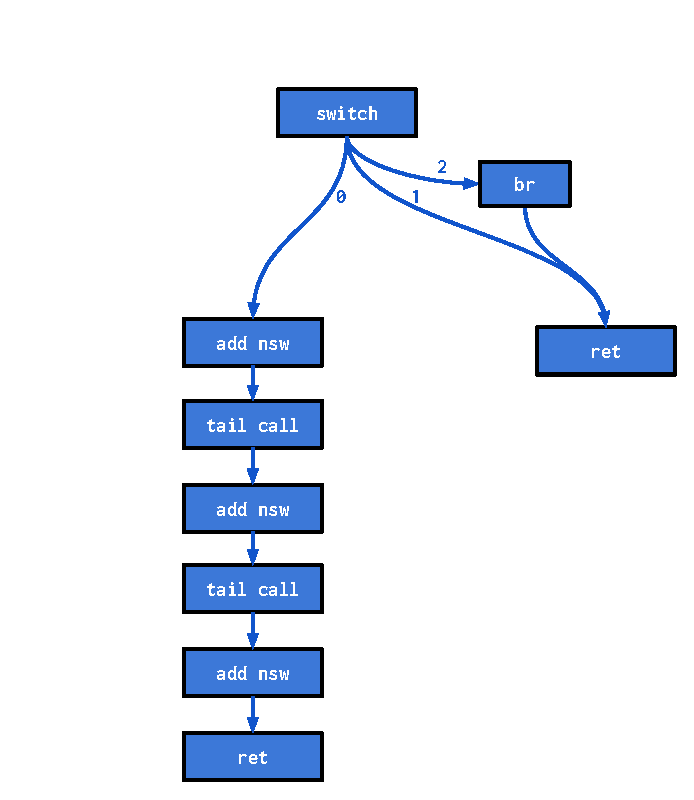
\includegraphics[width=\linewidth]{images/B_Control}%
    \caption{Construct control flow.}
    \label{subfigure:control_flow}%
  \end{subfigure}
  \\*
  \vspace{1em}
  \begin{subfigure}{.48\linewidth}%
    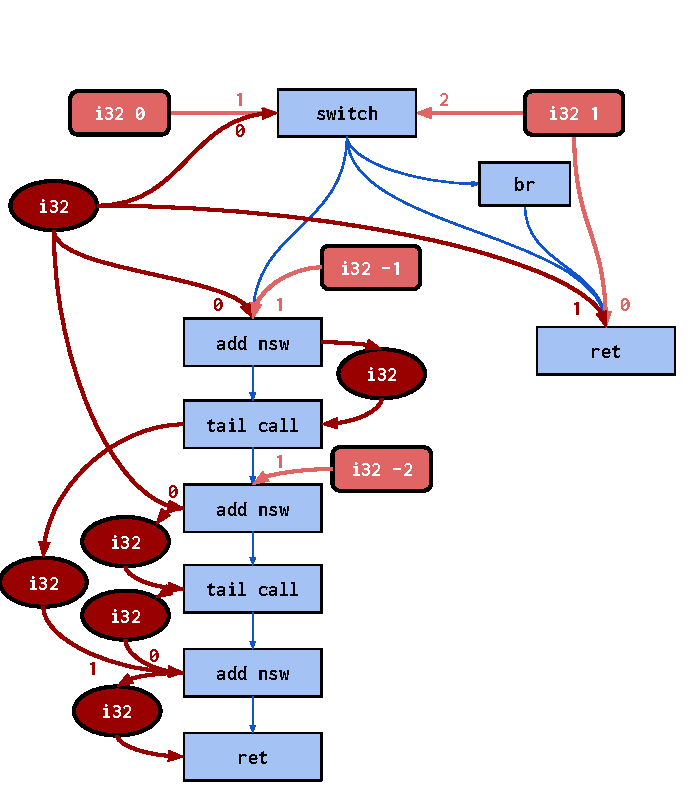
\includegraphics[width=\linewidth]{images/C_Data}%
    \caption{Add data flow for variables and constants.}
    \label{subfigure:data_flow}%
  \end{subfigure}
  \begin{subfigure}{.48\linewidth}%
    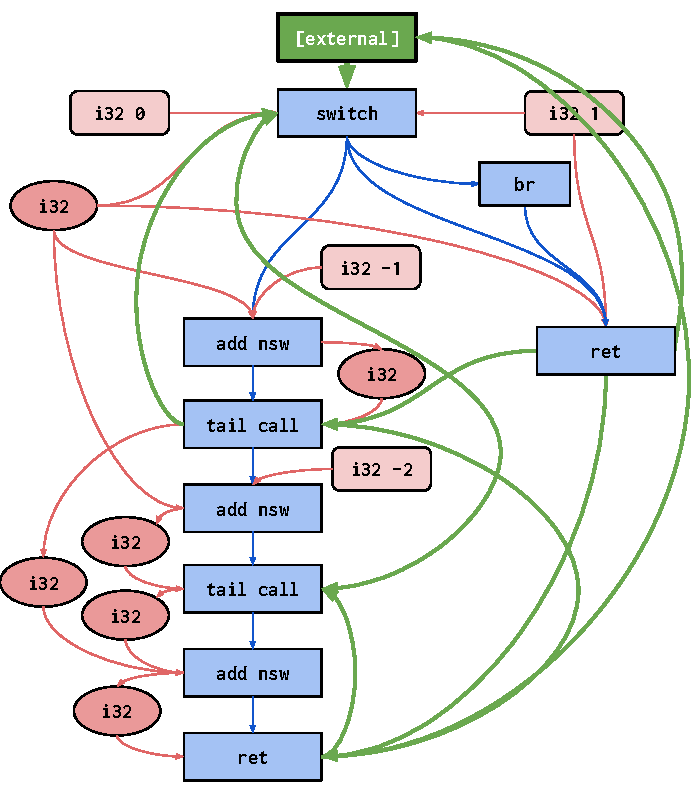
\includegraphics[width=\linewidth]{images/D_Call}%
    \caption{Add call flow for call sites.}
    \label{subfigure:call_flow}%
  \end{subfigure}
  \caption{%
    Construction of a \textsc{ProGraML} representation for a simple C
    implementation of recursive Fibonacci using LLVM-IR. The input
    program is passed through the compiler front end to produce an
    intermediate representation (a). A full flow graph is constructed
    from the IR statements and control flow edges inserted
    (b). Vertices for variables and constant values are  added and
    data-flow edges inserted (c). Finally, call sites are extracted
    and call edges inserted from call sites to function entry
    statements, and from function exit vertices to call sites (d). All
    edges are positional, for clarity we have omitted position labels
    where not required.%
  }%
  \label{figure:graph_construction}%
\end{figure*}

\subsection{Overview}

The \textsc{ProGraML} representation of a compiler IR serves as the
union between a call graph, control-flow graph, and data-flow
graph. We represent programs as directed multigraphs where statements,
identifiers, and immediate values are vertices, and relations between
vertices are edges. Edges are typed to differentiate control-, data-,
and call-flow. Additionally, we augment edges with a positional label
to encode the order of operands for statements, and to differentiate
between divergent branches in control-flow. The \textsc{ProGraML}
representation is processed natively by our machine learning models,
described in Section~\ref{sec:graph-based-machine-learning}.

\subsection{Graph Construction}

We construct a \textsc{ProGraML} graph $G = (V, E)$ by traversing a
compiler IR. Graph construction is divided into three stages:
control-flow, data-flow, and call-flow, though in practice the three
stages can be combined in a single $\bigo{(|V|+|E|)}$ pass. The
representation is compiler-agnostic, adding support for a new compiler
requires only a parser for the IR. Currently we support
LLVM~\cite{Lattner2004} and XLA HLO~\cite{Leary2017}
IRs. Figure~\ref{figure:graph_construction} shows the graph
construction approach.

\paragraph{(I) Control Flow} We construct a full-flow graph from an IR
by inserting a graph vertex for each instruction and control flow
edges between them, as shown in
Figure~\ref{subfigure:control_flow}. All control edges are augmented
with a numeric position label using an ascending sequence based on
their order in the list of a vertex's outgoing control edges. For
instructions with a single control successor, the position of the
control edge is 0. For a branching statement with $n$ successor
statements, the control edge positions are in the range
$0 \le e_{\text{pos}} \le n$. We do not need to encode the source
function or basic block~\cite{Lattner2004} of instructions as this
information is captured implicitly in structure of the graph; basic
blocks are regions of instructions with a single entry and exit
control edge, and functions are disconnected subgraphs.

\paragraph{(II) Data Flow} We introduce additional graph vertices for
constant values and variables, shown in
Figure~\ref{subfigure:data_flow}. Data-flow edges are added to capture
the relation from constants and variables to the instructions that use
them as operands, and instructions to produced variables. Each unique
variable and constant is a vertex, which implicitly models the scope
of variables, and unlike the tokenized representations of prior
machine learning works, variables in different scopes always map to
distinct vertices and can thus be discerned. Similarly, constant
values with the same textual representation in source code (such as
the number \texttt{3.14} with \texttt{float} and \texttt{double}
precision types) are distinguishable in our representation. As with
control edges, data edges have a position label which encodes the
order of operands for instructions. The latent representation of an IR
statement is thus a function of the vertex representing the
instruction and the vertices of any operand variables or constants,
modulated by their order in the list of operands.

\paragraph{(III) Call Flow} Control edges do not span functions, such
that an IR with functions $F$ produces $|F|$ disconnected subgraphs
(the same is not true for data edges which may cross function
boundaries, for example in the case of an global constant which is
used within multiple functions of a program). Instead, the relation
between a statement which calls a function and the called function is
captured through call edges, shown in
Figure~\ref{subfigure:call_flow}. An outgoing call edge is inserted
from the calling statement to the entry statement of a
function. Return call edges are added from all terminal statements of
a function to the calling statement. Call edges do not use position
labels as there is no ordering to be imposed between the call sites of
a function. For IRs which support external linkage, an additional
vertex is created representing an external callsite and connected to
all externally visible functions. Similarly, if a call site references
a function not defined in the current IR, a \emph{dummy} function
definition is created consisting of a pair of entry and exit
instruction vertices, and connected normally through call edges. A
single dummy function definition is created for each externally
defined function and shared across all call sites in the current IR.


\subsection{Comparison to Other Representations}

As an input for machine learning, what distinguishes \textsc{ProGraML}
from prior works is its close proximity to the structured
representations traditionally used within compilers for program
analysis and optimization. Specifically, it is distinct from prior
machine learning representations in three key areas:
\begin{enumerate}
\item as an IR-level representation, it is independent of the source
  language and accompanying variances such as code style and
  identifier naming that affect source-level
  representations~\cite{Alon2018a,Cummins2017a};
\item by representing programs as graphs with explicit control, data,
  and call edge types \textsc{ProGraML} captures a greater range of
  intra-program relations than prior graph
  representations~\cite{Ben-nun2018,Allamanis2017b,Park2012};
\item and in trading sequential for graph representations, we do not
  sacrifice local sequence order, such as the ordering of diverging
  control flow or the ordering of operands that is lost in prior
  representations~\cite{Ben-nun2018,Brauckmann2020}.
\end{enumerate}

Table~\ref{tab:representation_taxonomy} provides a comparison of
\textsc{ProGraML} to several recent learned representations of code.

\begin{table}
  \centering
  \footnotesize
  \begin{tabular}{r L{3.6cm} L{2.5cm} L{1.8cm} L{1.8cm} L{1.8cm}}
    \toprule
    & Source Languages & Representation & Flow-sensitive? & Position-sensitive? & Value-sensitive? \\
    \midrule
    AST Paths~\cite{Alon2018c} & C\#, Java, JavaScript, Python & AST & &  & \cmark \\
    CDFG~\cite{Brauckmann2020} & OpenCL & IR Graph & \cmark &  &  \\
    code2vec~\cite{Alon2018a} & Java & AST & & & \cmark \\
    DeepTune~\cite{Cummins2017b} & OpenCL & Token Sequence &  & \cmark & \cmark \\
    DeepTune-IR\cite{Barchi2019a} & OpenCL & IR Token Sequence &  & \cmark & \\
    DeepTyper~\cite{Hellendoorn2018} & JavaScript & Token Sequence &  & \cmark & \cmark \\
    inst2vec~\cite{Ben-nun2018} & C++, OpenCL & IR Graph & \cmark & & \cmark \\
    \textbf{\textsc{ProGraML}} & \textbf{C, C++, Fortran, Haskell, OpenCL, Swift} & \textbf{IR Graph} & \cmark & \cmark & \cmark \\
    \bottomrule
  \end{tabular}
  \vspace{.3em}
  \caption{%
    Taxonomy of recent code representations for machine learning. We
    classify approaches based on the type of representation used and
    the sensitivity to three categories: \{control/data/call\}-flow,
    operand positions, and operand values. Prior approaches require a
    trade-off in representational power, e.g. substituting a
    position-sensitive token sequence for a flow-sensitive
    graph. \textsc{ProGraML} is the first representation to span all
    categories.%
  }%
  \label{tab:representation_taxonomy}
\end{table}

\section{Graph-based Machine Learning for Program Analysis}
\label{sec:graph-based-machine-learning}

We formulate our system in a Message Passing Neural Network (MPNN)
framework~\citep{Gilmer2017}. Our design mimics the \emph{transfer functions}
and \emph{meet operators} of classical iterative data flow
analysis~\citep{Kam1977,Cooper2003}, replacing the rule-based implementations
with learnable analogues (message and update functions). This single unified
model can be specialized through training to solve a diverse set of problems
without human intervention or algorithm design.

The \programl model is an adaptation of GGNN~\citep{Li2015a} that takes as input
an attributed directed multigraph as presented in
Section~\ref{sec:graph-representation}. It consists of three logical phases:
input encoding, message propagation and update, and result readout.

\paragraph{(I) Input Encoding} Starting from the augmented graph representation
$G = (V, E)$, we capture the semantics of the program graph vertices by mapping
every instruction, constant, and variable vertex $v \in V$ to a vector
representation $h_v^0 \in \mathbb{R}^{d}$ by lookup in a fixed-size learnable
embedding table. The mapping from vertex to embedding vector $f: v \mapsto
h_v^0$ must be defined for each IR.

For LLVM-IR, we construct an embedding key from each vertex using the name of
the instruction, e.g., \texttt{store}, and the data type for variables and
constants, e.g., \texttt{i32*} (a pointer to a 32-bit integer). In this manner,
we derive the set of unique embedding keys using the graph vertices of a
training set of LLVM-IRs described in Section~\ref{subsec:dataset}. This defines
the embedding table used for training and deployment. An \emph{unknown element}
embedding is used during deployment to map embedding keys  which were not
observed in the training data. Since composite types make the size of the
vocabulary unbounded in principle, our data-driven approach trades a certain
amount of semantic resolution against good coverage of the vocabulary by the
available datasets (cf. Table 1). The embedding vectors are trained jointly with
the rest of the model.

\paragraph{(II) Message Propagation} Each iteration step is divided into a
message propagation  followed by vertex state update. Receiving messages
$M(h_w^{t-1}, e_{wv})$ are a function of neighboring states and the respective
edge. Messages are mean-aggregated over the neighborhood after transformation
with a custom position-augmented transfer function that scales $h_w$ elementwise
with a position-gating vector $p(e_{wv})$:%
\begin{equation*}
	M(h^{t-1}_w,e_{wv}) = W_{\mathrm{type}(e_{wv})} \Big(h_w^{t-1} \odot p(e_{wv})\Big) + b_{\mathrm{type}(e_{wv})}
\end{equation*}
The position-gating $p(e_{wv}) = 2 \sigma (W_p \operatorname{emb}(e_{wv}) +
b_p)$ is implemented as a sigmoid-activated linear layer mapping from a constant
sinusoidal position embedding ~\citep{Vaswani2017,Gehring2017}. It enables the
network to distinguish non-commutative operations such as division, and the
branch type in diverging control-flow. In order to allow for reverse-propagation
of information, which is necessary for backward compiler analyses, we add
backward edges for each edge in the graph as separate edge-types. In all our
experiments, we employ Gated Recurrent Units (GRU)~\citep{Cho2014} as our update
function.

Step (II) is iterated $T$ times to extract vertex representations that are
contextualized with respect to the graph structure.

\paragraph{(III) Result Readout} Data flow analyses compute value sets composed
of instructions or variables. We support per-instruction and per-variable
classification tasks using a \emph{readout head} on top of the iterated feature
extraction, mapping, for each vertex, the extracted vertex features $h_v^T$ to
probabilities $R_v(h_v^T, h_v^0)$:
\begin{equation*}
	R_{v}(h_v^T, h_v^0) = \sigma\left(f(h_v^T, h_v^0)\right) \cdot g(h_v^T) \\
\end{equation*}
where $f(\cdot)$ and $g(\cdot)$ are linear layers and $\sigma(\cdot)$ is the
sigmoid activation function. Allowing the readout head to access the initial
node state $h_v^0$ in its gating function $\sigma(f(\cdot))$ acts as a skip
connection from the input embedding to the readout.

\section{Experimental Methodology}%
\label{sec:methodology}

We evaluate the effectiveness of our approach in three case
studies. In the first, we apply our methodology to a suite of
established compiler analysis tasks. These serve as demonstrations of
the representational power of our approach and highlight the
limitations both in prior machine learning approaches and in current
MPNNs. The second case study then applies the approach to the
challenging real-world optimization task of heterogeneous device
mapping, comparing the performance of our model against
state-of-the-art machine learning-based approaches. Finally, we apply
our approach to the task of classifying algorithms from unlabelled
implementations. This section describes the methodology used to
construct these experiments: the datasets used, the model parameters,
and training regimes.


\subsection{Case Study A: Compiler Analyses}

We construct a benchmark suite of traditional compiler analysis tasks
to evaluate the representational power of our approach.  We chose a
diverse set of tasks to capture a mixture of both forward and backward
analyses, and control-, data-, and procedure-sensitive analyses. Our
goal is not to suggest that machine learning should replace the
existing implementations of these standard algorithms which can be
found in any compiler, but rather, if a machine learning system is
\emph{not} capable of producing these analyses, it stands to reason
that performance on downstream tasks which depend on these analyses
will suffer.

\subsubsection{Benchmark Analyses}

We selected five traditional compiler analyses to use as benchmarks
for evaluating the representational power of our approach.

\paragraph{(I) Reachability} Control reachability is a fundamental
compiler analysis which determines the set of statements that can be
reached from a particular starting statement. Given $\text{succ}(n)$,
which returns the control successors of statement $n$, the set of
reachable statements starting at root $n$ can be found using forward
analysis:

\begin{equation}
  \text{Reachable}(n) = \{n\} \cup \left( \bigcup_{s \in \text{succ}(n)} \text{Reachable}(s) \right)
\end{equation}

\paragraph{(II) Dominator trees} Statement $n$ dominates statement $m$
if every control flow path to $m$ passes through $n$. A dominator tree
is the set of all nodes that dominate the statment at a particular
program point. Like reachability, this analysis only requires
propagation of control flow, but unlike reachability, dominator trees
are typically constructed using backward
analysis~\cite{Lengauer1979,Blazy2015}:

\begin{equation}
  \text{Dominators}(n) = \{n\} \cup \left( \bigcap_{p \in \text{pred}(n)} \text{Dominators}(p) \right)
\end{equation}

Where $\text{pred}(n)$ which returns the control predecessors of
statement $n$.

\paragraph{(III) Live-out variables} A variable $a$ is live-out of
statement $n$ if there exists some control successor of $n$ that uses
$a$. Given $\text{uses}(n)$, which returns the operand variables of
$n$, and $\text{defs}(n)$, which returns defined variables, the
live-out variables can be computed forwards using:

\begin{equation}
  \text{LiveOut}(n) = \bigcup_{s \in \text{succ}(n)} \text{uses}(s) \cup \big(  \text{LiveOut}(s) - \text{defs}(s) \big)
\end{equation}

\paragraph{(IV) Data dependencies} The data dependencies of statement
$n$ is the set of predecessor statements that must be evaluated to
produce the operands of $n$. Computing data dependencies requires data
sensitivity and is computed backwards:

\begin{equation}
  \text{DataDep}(n) = \text{defs}(n) \cup \left( \bigcup_{p \in \text{defs}(n)} \text{DataDep}(p) \right)
\end{equation}

Where $\text{defs}(n)$ returns the statements that produce operands of
$n$.

\paragraph{(V) Global Common Subexpressions} The identification of
common subexpressions is an important analysis for optimization. For
compiler IRs we define a subexpression as a statement and its
operands, ordered by either their position (for non-commutative
operations), or lexicographically (for commutative operations). We
thus formulate the common subexpression problem as, given a statement
(which forms part of a subexpression), label any other statements in
the program which compute the same subexpression. This is an
inter-procedural analysis, though operands must obey their
scope. Common subexpressions are typically identified using available
expression analysis:

\begin{equation*}
\text{Avail}(n) = \text{uses}(n) \cup \left( \bigcap_{p \in \text{pred}(n)} \text{Avail}(p) \right) - \text{defs(n)}
\end{equation*}

Where $\text{uses}(n)$ return the expressions used by statement $n$,
and $\text{defs}(n)$ returns the expressions defined by $n$.


\subsubsection{Datasets}

We assembled a large corpus of real-world LLVM-IRs from a variety of
sources, summarized in Table~\ref{table:corpus}. We selected popular
open source software projects that cover a diverse range of domains
and disciplines, augmented by uncategorized code mined from popular
GitHub projects using the methodology described by Cummins et
al.~\cite{Cummins2017a}. Our corpus comprises a range of source
languages (C, C++, Fortran, Haskell, OpenCL, and Swift) and exceeds
250k files. We de-duplicated the corpus first at the source level,
then again after lowering to LLVM-IR. Lowering from source to IR was
performed using the inst2vec methodology~\cite{Ben-nun2018}, in which
an optimization level is chosen randomly per-file.

\begin{table}
  \centering%
  \renewcommand{\arraystretch}{1.55}
\footnotesize
\begin{tabular}{L{3.35cm} L{1.45cm} L{2.75cm} | r r R{1.69cm} R{1.6cm}}
  & \textbf{Source language} & \textbf{Domain} & \textbf{IR files} & \textbf{IR lines} & \textbf{Avg. vertices / IR} & \textbf{Avg. edges / IR}\\
  \hline
  BLAS 3.8.0 & Fortran & Scientific Computing & 300 & 345,613 & 1,664 & 3,276\\
  \hline
  Linux 4.19 & C & Operating Systems & 13,851 & 41,332,089 & 1,857 & 3,760 \\
  \hline
  OpenCL Benchmarks~\cite{Cummins2017b} & OpenCL & Benchmarks & 256 & 149,779 & 1,027 & 1,970 \\
  \hline
  OpenCV 3.4.0 & C++ & Computer Vision & 400 & 1,168,758 & 3,761 & 7,442\\
  \hline
  POJ-104~\cite{Mou2016} & C++ & Standard Algorithms & 182,815 & 64,518,837 & 312 & 569 \\
  \hline
  Tensorflow~\cite{Abadi} & C++ & Machine learning & 1,584 & 8,444,443 & 5,786 & 11,482 \\
  \hline
  \multirow{4}{*}{GitHub} & C & \multirow{4}{*}{Various} & 42,880 & 89,356,570 & 927 & 1,794\\
                  & Haskell & & 1,371 & 6,745,312 & 4,705 & 7,518\\
                  & OpenCL & & 5,188 & 10,472,388 & 2,299 & 5,132 \\
                  & Swift & & 1,783 & 205,140 & 134 & 371 \\
  \hline
  \textbf{Total} & --- & --- & \textbf{250,428} & \textbf{222,738,929} & \textbf{153,426,059} & \textbf{294,685,614} \\
  \hline
\end{tabular}
%
  \vspace{.5em}
  \caption{%
    The ten sources of LLVM-IR used to produce datasets for evaluating
    data flow analyses. Our corpus comprises six programming languages
    from functional to imperative, high-level to accelerators. The
    software covers a broad range of disciplines from compilers and
    operating systems to traditional benchmarks, machine learning
    systems, and unclassified code downloaded from popular open source
    repositories.%
  }%
  \label{table:corpus} %
\end{table}

We generated a single \textsc{ProGraML} representation for each of the
LLVM-IRs, taking an average of 31 ms per IR. Our corpus of unlabeled
graphs totals 153M vertices and 295M edges, with an average of 616
vertices per graph with 472 unique vertex representations, and 1183
edges with a maximum edge position of 355 (a large \texttt{switch}
statement found in a Tensorflow compute kernel).

We produced labeled graphs from the unlabeled corpus by computing
ground truth labels for each of the analysis tasks using a traditional
analysis implementation.  For each of the five tasks, and for every
unlabeled graph in the corpus, we produce $n$ labeled graphs by
selecting unique source vertices $v_{0} \in V$, where $n$ is
proportional to the size of the graph:
\begin{equation}
n = \min \left( \left\lceil \frac{|V|}{10} \right\rceil, 10 \right)
\end{equation}
Each instance in the datasets consists of an input graph in which the
source vertex is indicated using the \emph{vertex selector}, and an
output graph with the ground truth labels used for training or for
evaluating the accuracy of model
predictions. Figure~\ref{fig:dataflow_examples} illustrates an example
input-output instance for each of the five tasks.

We divided the datasets randomly using a 3:1:1 ratio for training,
validation, and test instances. The same random allocation of
instances was used for each of the five tasks. Where multiple labeled
graphs were derived from a single IR, instances derived from the same
IR were allocated to the same split.

\begin{figure}
  \centering
  \begin{subfigure}{.19\linewidth}
    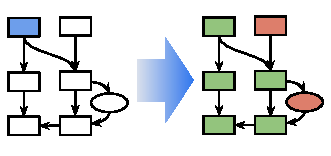
\includegraphics[width=\linewidth]{images/dataflow/A_reachability}%
    \caption{\textsc{Reachability}.}
    \label{subfig:dataflow_reachability}
  \end{subfigure}
  \hfill
  \begin{subfigure}{.19\linewidth}
    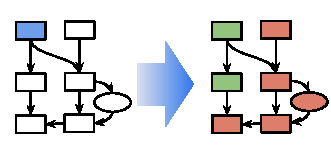
\includegraphics[width=\linewidth]{images/dataflow/B_domtree}%
    \caption{\textsc{Domtree}.}
    \label{subfig:dataflow_domtree}
  \end{subfigure}
  \hfill
  \begin{subfigure}{.19\linewidth}
    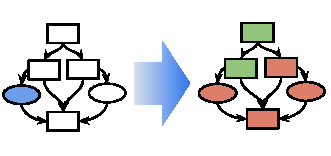
\includegraphics[width=\linewidth]{images/dataflow/C_datadep}%
    \caption{\textsc{DataDep}.}
    \label{subfig:dataflow_datadep}
  \end{subfigure}
  \hfill
  \begin{subfigure}{.19\linewidth}
    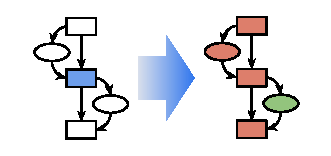
\includegraphics[width=\linewidth]{images/dataflow/D_liveness}%
    \caption{\textsc{Liveness}.}
    \label{subfig:dataflow_liveness}
  \end{subfigure}
  \hfill
  \begin{subfigure}{.19\linewidth}
    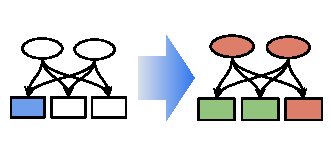
\includegraphics[width=\linewidth]{images/dataflow/E_subexpressions}%
    \caption{\textsc{Subexpressions}.}
    \label{subfig:dataflow_subexpressions}
  \end{subfigure}
  \caption{%
    Example input-output graphs for each of the five benchmark
    compiler analyses. A single vertex is randomly selected from the
    input graph to represent the starting program for computing the
    analysis results, indicated using the \emph{vertex selector}. The
    output graphs contain binary labels for each of the graph vertices
    after the analysis has completed. As a supervised classification
    task, the goal of the model is to predict the output vertex labels
    given the input graph. These small graphs are for illustrative
    purposes, the LLVM-IR graphs in our real-world corpus contain an
    average 616 vertices and 1,183 edges.%
  }%
  \label{fig:dataflow_examples}%
\end{figure}

\subsubsection{Models}%
\label{subsubsec:dataflow_models}

\paragraph{LSTM Baseline} As no prior work offers the expressiveness
required to perform the per-statement and per-variable classification
required for these analysis tasks, we extended
DeepTune~\cite{Cummins2017b}, a state-of-the-art deep learning
framework for whole-program classification, to enable per-statement
classification. In DeepTune, an OpenCL program is first tokenized and
mapped to a sequence of embedding vectors which are then processed
through a sequential LSTM model. The final state of the LSTM is
optionally concatenated with program-level features, then fed through
a fully connected neural network to produce a program-level
classification.

Figure~\ref{figure:lstm_node_level} shows how we extended this
approach for statement-level classification of LLVM-IR. We first
replaced the OpenCL tokenizer using one derived from LLVM IR,
resulting in a 179-element vocabulary. To adapt the approach for
performing statement-level classification, we group embedding vectors
by their source statement before using element-wise summation to merge
embedding vectors.

We use the same models parameters as in the original
work~\cite{Cummins2017b} --- 64-dimensional embedding vectors trained
jointly, with 64 sequences per batch, padded and truncated to the same
length. As LLVM IR is more verbose than OpenCL, the sequences are
significantly longer requiring greater device memory during training
and inference. This is a common issue with recurrent neural networks,
as sufficient memory is required to store both the intermediate
results of the forward pass and the gradients during
training~\cite{Ben-Nun2019a}. We found that a sequence length of 5,000
was the maximum that our experimental platform allowed. Where
sequences exceed this length, they are truncated, and the model
outputs padded with zeros to match the expected shape.


\begin{figure}
    \centering %
    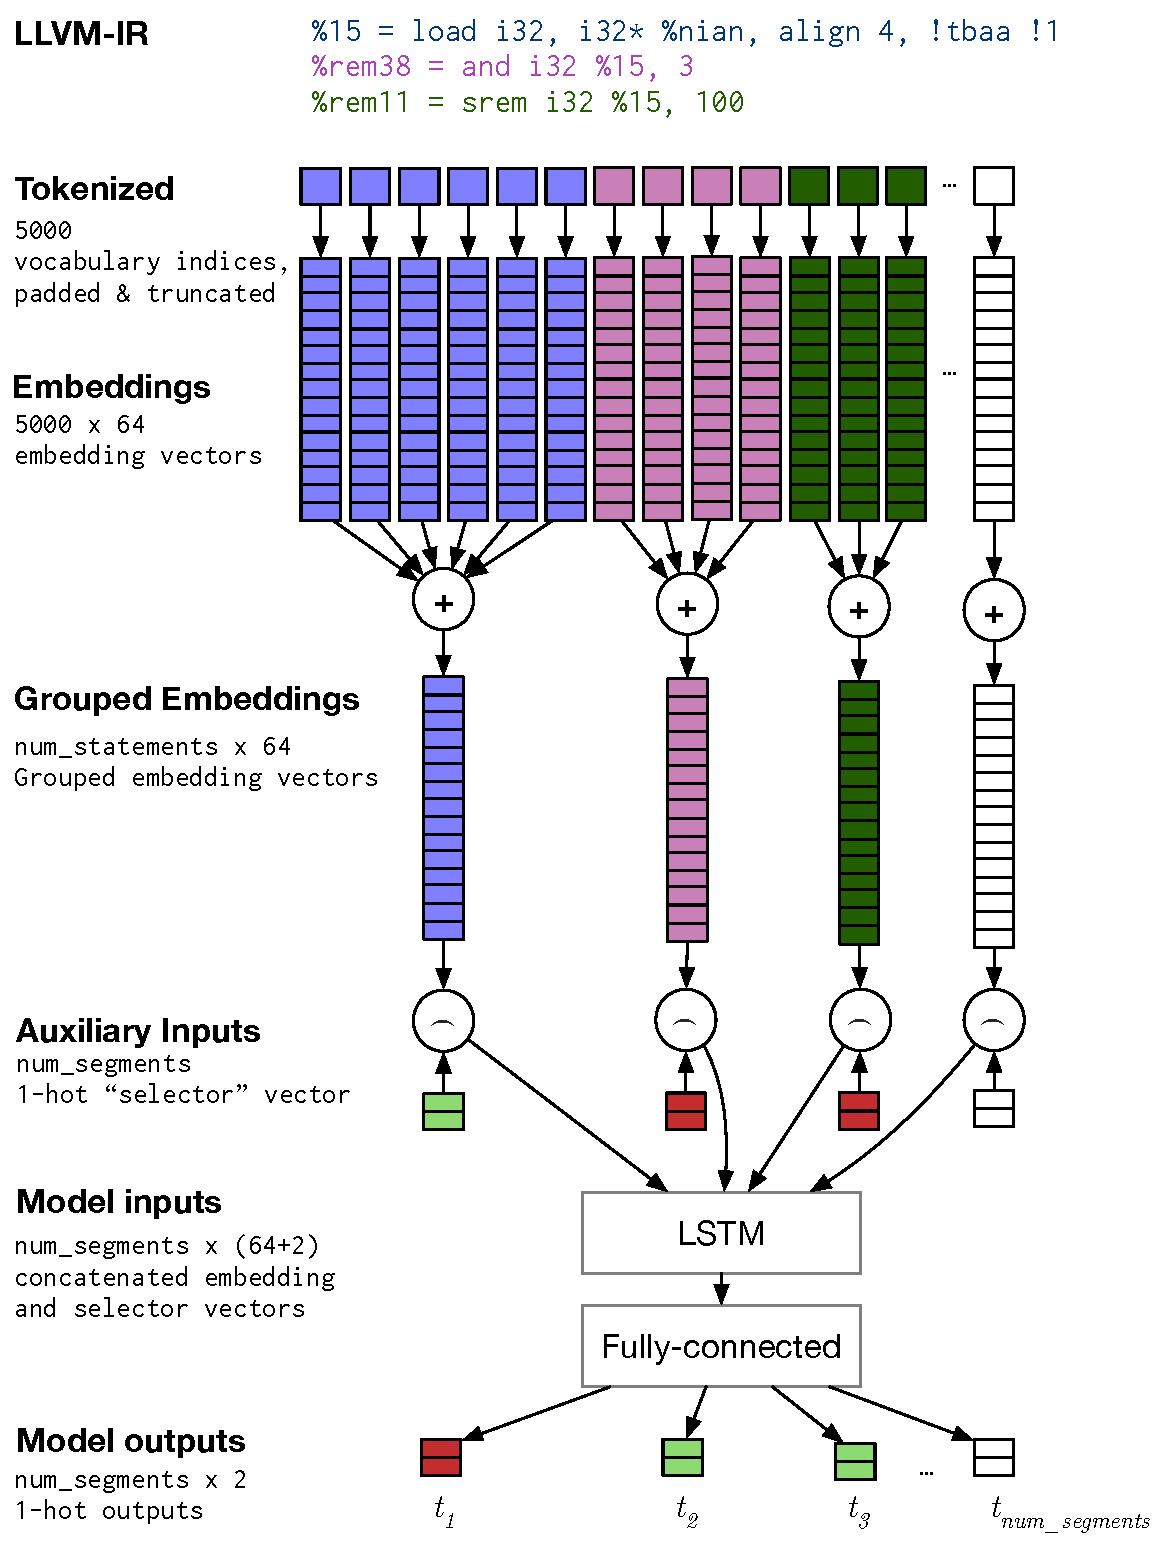
\includegraphics[width=.62\columnwidth]{images/lstm_node_level}%
    \caption{%
      Extending DeepTune~\cite{Cummins2017b} to perform per-statement
      classification of an LLVM-IR. In the original work, the latent
      representation of the entire program token sequence was used for
      program-level classification, we enable classification of
      arbitrary token groupings so that we can perform statement-level
      classification of a program. In the above diagram, $+$ denotes
      element-wise summation, and $\frown$ denotes vector
      concatenation.%
    }%
    \label{figure:lstm_node_level}%
\end{figure}

\paragraph{ProGraML} We use the model design outlined in
Section~\ref{sec:graph-based-machine-learning} for each of the
compiler analysis tasks. While we use the vocabulary of inst2vec, we
do not use the pre-trained embeddings, instead initializing the
embeddings randomly and training jointly.

Message Passing Neural Networks typically use a small number of
propagation steps out of practical consideration for time and space
efficiency~\cite{Gilmer2017,Li2015a}, and address problems on smaller
graphs than used in this work~\cite{Allamanis2017b}. For a large class
of monotone data flow analysis problems, however, it is known that up
to $d(G) + 3$ passes over the graph are required, where $d(G)$ is the
\emph{loop connectedness} of $G$~\cite{Cooper2003,Kam1977}.  The
\emph{loop connectedness} captures the notion of loop-nesting depth in
a program and is therefore a program-dependent, but generally
unbounded quantity\footnote{Given any depth-first spanning tree (DFST)
  of $G$, backward edges are defined as edges in $G$ that connect a
  node to one of its ancestors in the DFST and $d(G)$ is the maximum
  number of backwards edges in any acyclic path in $G$.}.

We address this challenge with \textsc{ProGraML} by iterating for a
fixed number $T$ of message passing steps for training and inference
and excluding from the test set graphs for which a traditional
implementation of the analysis task requires greater than $T$
iterations to solve. For the experiments in this work we set $T = 30$,
leading to 12.56\% of the graphs in the corpus to be excluded across
the five tasks. For fairness, we also excluded these graphs from
evaluation of the LSTM baseline.


\subsubsection{Training Details and Parameters}
All models were trained in an end-to-end fashion with the Adam
optimizer \cite{Kingma2015} using the default configuration and
learning rate $0.001$. We trained the models on a NVIDIA GTX 1080
GPU-equipped machine in increments of 10k graphs, testing on a 20k
validation set at each checkpoint. Training terminated after six
hours, or if accuracy on the validation set reached 99.99\%. After
training completed we selected the checkpoint with the highest
accuracy on the validation set to use for testing.


\subsection{Case Study B: Heterogeneous Device Mapping}

We apply our methodology to the challenging domain of heterogeneous
device mapping (\textsc{DevMap}). Given an OpenCL kernel and a choice
of two devices to run it on (CPU or GPU), the \textsc{DevMap} task is
to predict the device which will provide the best performance. We
chose this problem as it has received significant prior attention,
with previous approaches using both hand-engineered
features~\cite{Grewe2013} and sequential models~\cite{Cummins2017b,
  Ben-nun2018}.

\subsubsection{Datasets}

We used the dataset of~\cite{Cummins2017b}, which provides labeled
CPU/GPU instances for 256 OpenCL kernels sourced from seven benchmark
suites on two combinations of CPU/GPU pairs. The \emph{AMD} set uses
an Intel Core i7-3820 CPU and AMD Tahiti 7970 GPU; the \emph{NVIDIA}
set uses an Intel Core i7-3820 CPU and an NVIDIA GTX 970 GPU. Each
dataset consists of 680 labeled instances derived from the 256 unique
kernels by varying dynamic inputs.

\subsubsection{Models}%
\label{subsubsection:devmap_models}

We compare ProGraML with four approaches: First, with a static
baseline that predicts the mode device of the dataset
distribution. Second, with DeepTune~\cite{Cummins2017b}, which is a
sequential LSTM model at the OpenCL source level. Third, to isolate
the impact of transitioning from OpenCL source to LLVM-IR, we evaluate
against a new DeepTune$_{\text{IR}}$ model, which adapts DeepTune to
using tokenized sequences of LLVM-IR as input instead of OpenCL
tokens, using the vocabulary described in
Section~\ref{subsubsec:dataflow_models}. Finally, we compare against
the state-of-the-art approach NCC~\cite{Ben-nun2018}, which replaces
the OpenCL tokenizer with a sequence of 200-dimensional embeddings,
pre-trained on a large corpus of LLVM-IR using a skip-gram model.


\subsubsection{Training Details and Parameters}

All neural networks are regularized with Dropout \cite{Hinton2012} for
generalization and Batch Normalization \cite{Ioffe2015a} in order to
be uniformly applicable to vastly different scales of auxiliary input
features. We used $10$-fold cross-validation with rotating 80/10/10
splits by training on 80\% of the data and selecting the model with
the highest validation accuracy, setting aside $1/10$th of the
training data to use for validation. We trained each model for 100
epochs and selected the epoch with the greatest validation accuracy
for testing.


\subsection{Case Study C: Algorithm Classification}

In a third case study, we apply our approach to task of classifying
algorithms. We use the POJ-104~\cite{Mou2016} dataset.  It contains
implementations of 104 different algorithms that were submitted to a
judge system. All programs were written by students in higher
education. The dataset has around 500 samples per algorithm. We
compile them with different combinations of optimization flags to
generate a dataset of overall 240k samples. Approximately 10,000 files
are held out each as a development and test set.


\subsubsection{Models}

We compare with recently published tree-based convolutional neural
networks (TBCNN)~\cite{Mou2016} and NCC~\cite{Ben-nun2018}, which uses
the same approach approach as described in
Section~\ref{subsubsection:devmap_models} on this dataset. To further
test the expressive power of the graph-based representation against
the tree-based (TBCNN) and sequential (NCC) prior work, we present
additional experiments: Graph-based baselines based on
XFG~\cite{Ben-nun2018} and a \textsc{ProGraML} \emph{structure-only}
baseline.

To better understand the qualitative aspects of replacing a
graph-based representation that captures program semantics like
Contextual Flow Graphs~\cite{Ben-nun2018} (XFG) with the more complete
\textsc{ProGraML} representation, we adapted a GGNN~\cite{Li2015a} to
directly predict algorithm classes from XFG representations of the
programs. In contrast to this, Ben-Nun et al.~\cite{Ben-nun2018} used
XFG only to generate statement contexts for use in skip-gram
pre-training. Here, we lift this graphical representation and make it
accessible to a deep neural network directly, as opposed to the
structureless sequential approach in the original work (NCC).

Additionally, we include a \emph{structure-only baseline} of our
\textsc{ProGraML} approach, where only the type of each node
(instruction, variable, or constant) is encoded, refraining completely
from tokenizing statements. We think that algorithm classification is
a problem that lends itself especially well to judging the power of
the representation \emph{structure}, since most algorithms are
well-defined independent of implementation details such as datatypes.

To test the limits of the expressivity of \textsc{ProGraML}, combine
our representation with a powerful 10-layer
Transformer~\cite{Vaswani2017} encoder model, adapted as a graph
neural network for attributed graphs. We induce graph structure by
masking the attention scores in the self-attention layer with the
adjacency matrix of the \textsc{ProGraML} graphs. A new
space-efficient sparse implementation allows processing of graphs with
on the order of $10^5$ vertices. Different edge types are encoded by
introducing separate \emph{key} and \emph{value} projection matrices
into the self-attention layer~\cite{Vaswani2017,Fisches2020}.


\subsubsection{Training Details and Parameters}

The GGNN models were trained with the AdamW~\cite{Loshchilov2019}
optimizer with learning rate
$2.5\cdot 10^{-4}, \beta_1=0.9, \beta_2=0.999, \varepsilon=10^{-8}$
for 80 epochs. Dropout regularization is employed on the graph states
with a rate of $0.2$. The Transformer model uses the same
hyperparameters as the GGNN. Additionally a batch size of 64, Dropout
regularization of 0.2 on the graph states and weight-sharing between
adjacent pairs of layers is employed. The model dimension is equal to
the embedding size (200) and the hidden size of the feed-forward
layers is 512. The self-attention layers use 5
heads~\cite{Vaswani2017}. Overall, the Transformer model has 5.6
million trainable parameters, around 1.7 million of which are in the
embedding layer.

\section{Experimental Results}

This section evaluates the performance and limitations of our approach
for the three case studies described in Section~\ref{sec:methodology},
and provides a comparison to state-of-the-art approaches. First we
show that \textsc{ProGraML}, unlike prior state-of-the-art approaches
to machine learning over code, is capable of replicating core compiler
analysis tasks that are key to optimization. Second, we improve upon
prior approaches to the task of heterogeneous device mapping. Finally,
we set a new state of the art in the difficult task of classifying
program algorithms, and ablate the contribution of the structure and
content of the \textsc{ProGraML} representation.


\subsection{Case Study A: Compiler Analysis}

Table~\ref{table:data_flow_results} summarizes the performance of the
\textsc{ProGraML} approach when tasked with learning a suite of
benchmark compiler analysis, along with the performance of a
state-of-the-art sequential approach, DeepTune$_\text{IR}$. As a
binary classification task, compiler analyses display an extreme class
imbalance as only a small fraction of a program graph is typically
relevant to computing the result set of an analysis. On our datasets,
an accuracy of 96.6\% can be achieved by always predicting the
negative class. For this reason we report only binary precision,
recall, and $F_1$ scores with respect to the positive class.

\begin{table}
  \centering%
  \vspace{.5em}
\footnotesize
\begin{tabular}{l L{4cm} r c c | c : c c}
  Analysis & Example Optimization &  & inst2vec & CDFG & \multicolumn{3}{c}{\programl} \\
   & & & DDF-30  & DDF-30 & DDF-30 & DDF-60 & \ddfinf{}\\
  \toprule
Reachability &
\multirow{2}{2.1cm}{Dead Code Elimination}
        & Precision  &  0.105  & \textbf{1.000}  &  0.998 & 0.997 & 0.996  \\
       & & Recall  &  0.007  & 0.996  &  \textbf{0.998}  & 0.998 & 0.917 \\
  \vspace{.3em}
        & & F$_1$  &  0.012  & \textbf{0.998}  &  \textbf{0.998} & 0.997 & 0.943 \\
Dominance &
Global Code Motion
        & Precision  &  0.053  &  0.999  &  \textbf{1.000} & 0.983 & 0.066 \\
       & & Recall  &  0.002  &  \textbf{1.000}  &  \textbf{1.000} & 1.000 & 0.950 \\
  \vspace{.3em}
        & & F$_1$  &  0.004  &  0.999  &  \textbf{1.000} & 0.991 & 0.123 \\
DataDep &
Instruction Scheduling
        & Precision  &  ---    &  ---    &  \textbf{0.998} & 0.992 & 0.987 \\
       & & Recall  &  ---    &  ---    &  \textbf{0.997} & 0.996 & 0.949 \\
  \vspace{.3em}
        & & F$_1$  &  ---    &  ---    &  \textbf{0.997} & 0.993 & 0.965 \\
Liveness &
Register Allocation
        & Precision  &  ---    &  ---    &  \textbf{0.962} & 0.931 & 0.476 \\
       & & Recall  &  ---    &  ---    &  \textbf{0.916} & 0.955 & 0.925 \\
  \vspace{.3em}
        & & F$_1$  &  ---    &  ---    &  \textbf{0.937} & 0.939 & 0.625 \\
Subexpressions &
\multirow{3}{3cm}{Global Common Subexpression Elimination}
        & Precision  &  0.000  &  0.139   &  \textbf{0.997}  & 0.954 & 0.938 \\
       & & Recall  &  0.000  &  0.005  &  \textbf{0.996}  & 0.999 & 0.992 \\
       & & F$_1$  &  0.000  &  0.009   &  \textbf{0.996} & 0.967 & 0.959 \\
\end{tabular}
\vspace{-1em}
%
  \vspace{.7em}
  \caption{%
    Benchmark compiler analyses results using two approaches: (a)
    DeepTune$_{\text{IR}}$, a sequential model adapted to work at the
    LLVM-IR level for statement-level classification, and (b)
    \textsc{ProGraML}, our approach. The relational representation
    significantly outperforms a sequential approach across all
    problems. For the Global Common Subexpressions analysis,
    DeepTune$_{\text{IR}}$ achieved a higher precision than
    \textsc{ProGraML} by predicting only the root statement as a
    component in a subexpression, avoiding false-positives.\\*
  }%
  \label{table:data_flow_results} %
\end{table}

As can be seen in Table~\ref{table:data_flow_results}, the relational
representation of our approach, coupled with learning through
iterative message passing, yields models that far outperform the
state-of-the-art sequential approaches to modeling code.  The grouping
of program tokens by statement performed by DeepTune$_\text{IR}$
offers a more restrictive classification interface than with
\textsc{ProGraML} (where data elements are also represented as graph
vertices). As such, it is not able to perform the per-variable
classification required for \textsc{Liveness}
analysis\footnote{Theoretically the same approach for grouping
  embeddings by statement could also be extended to group all
  statements by variables, but this would require duplicating many
  statements in the input representation, increasing the length of the
  sequences far beyond what we can practically process using a
  sequential model.}. For fairness, we exclude \textsc{Liveness} from
LSTM aggregate values in Table~\ref{table:data_flow_results}. Despite
this, \textsc{ProGraML} achieves an average 94.0 $F_1$, versus 27.3
$F_1$ for DeepTune$_\text{IR}$.

In many cases, the sequential model regresses to a classification mode
in which only the source vertex is labeled as positive, yielding poor
recall.  The \textsc{ProGraML} models achieve both high precision and
high recall in all tasks except \textsc{DomTree}, where recall is
comparatively poor. When model performance is considered as a function
of the number of training graphs, as shown in
Figure~\ref{fig:dataflow_convergence}, we see that the performance of
the \textsc{ProGraML} models quickly convergences towards near-perfect
$F_1$ score on a holdout validation set, except in the case of
\textsc{DomTree}, where the model is still improving at the end of
training. This suggests estimating the \emph{transfer} and \emph{meet}
operators of this backwards analysis poses a greater challenge for the
network, which may require further training.

\begin{figure}
  \begin{subfigure}{\linewidth}
    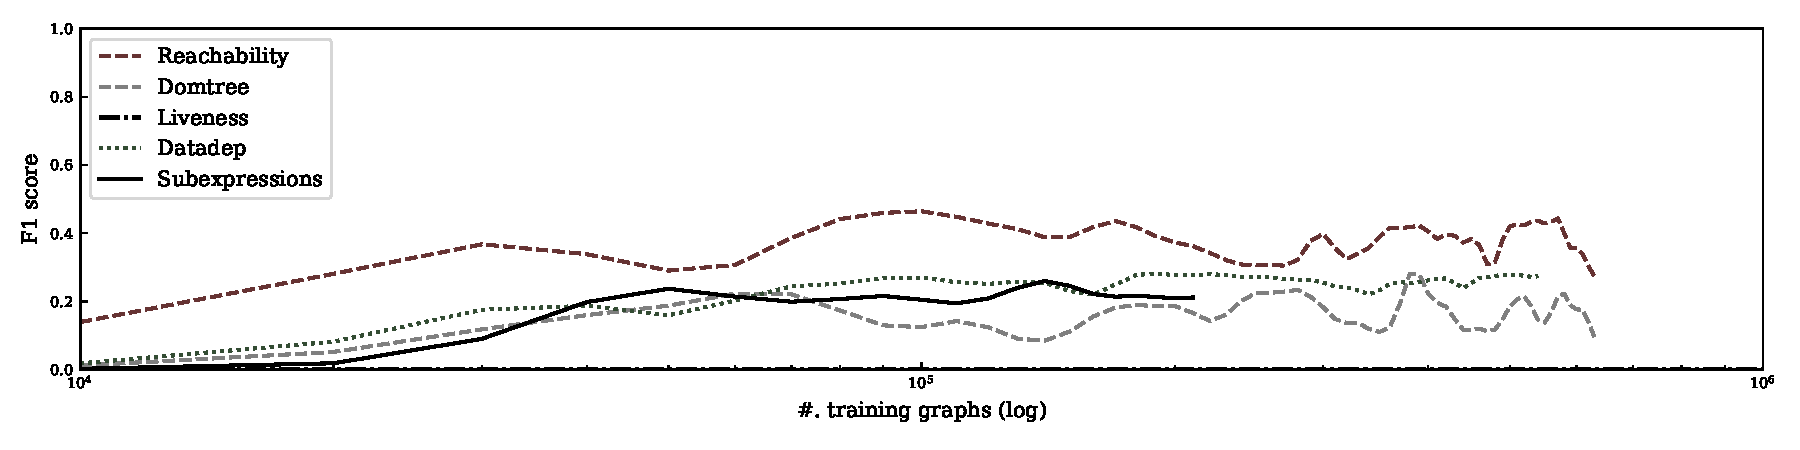
\includegraphics[width=\linewidth]{images/dataflow-lstm.pdf}
    \caption{DeepTune$_{\text{IR}}$}
    \label{fig:dataflow-lstm-f1}
  \end{subfigure}
  \\*
  \begin{subfigure}{\linewidth}
    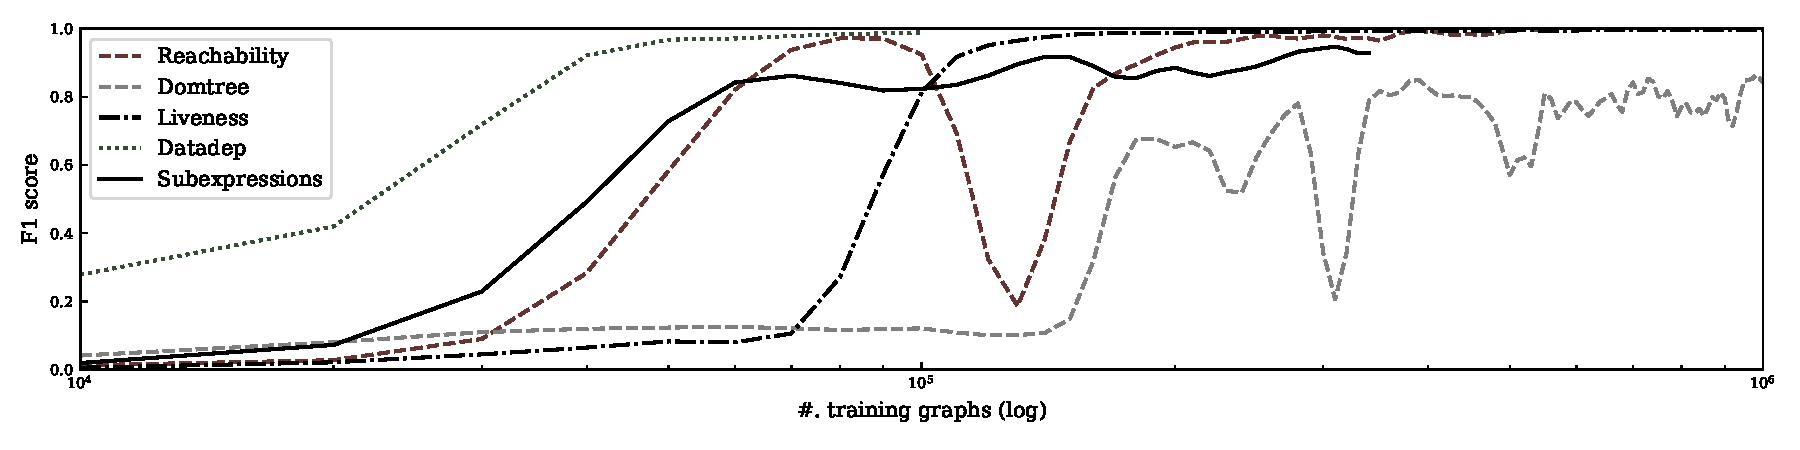
\includegraphics[width=\linewidth]{images/dataflow-ggnn.pdf}
    \caption{\textsc{ProGraML}}
    \label{fig:dataflow-ggnn-f1}
  \end{subfigure}
  \caption{%
    The $F_1$ score of compiler analysis models on a 20k-graph
    validation set as a function of the number of training graphs from
    10k to 1M. Each model was given six hours to train on a machine
    with a GTX 1080 GPU, with early termination if accuracy on the
    validation set reached 99.99\%. We have applied a Gaussian filter
    ($\sigma=1$) to aid in visualizing the trends in each set of
    scores.  }
  \label{fig:dataflow_convergence}
\end{figure}

Table~\ref{tab:confusion_matrices} shows confusion matrices for the
per-vertex classification of \textsc{ProGraML} models on the test
set. While the distribution of errors is balanced for
\textsc{Reachability}, in the case of \textsc{Domtree} and
\textsc{Subexpressions} the ratio of false negatives ($T_+P_-$)
outweighs the false positives ($T_-P_+$), indicating that models favor
under-approximating the value sets of these analyses. This may be an
artifact of training with such a large imbalance towards negatives
($T_-$) over positive ($T_+$) class labels. In future work we will
explore addressing this class imbalance by selecting multiple root
points on a graph for analysis simultaneously, thereby increasing the
size of the value set to include multiple (possibly overlapping)
regions.

\begin{table}
  \centering
\scriptsize
\renewcommand{\arraystretch}{1.5}
\begin{subfigure}{.19\linewidth}
  \centering
  \begin{tabular}{r | c c}
    \toprule
    & $\bm{P_-}$ & $\bm{P_+}$ \\
    \midrule
    $\bm{T_-}$ & 96.64\% & 0.01\% \\
    $\bm{T_+}$ & 0.01\% & 3.34\% \\
    \bottomrule
  \end{tabular}
  \caption{\textsc{Reachability}}
\end{subfigure}
\hfill
\begin{subfigure}{.19\linewidth}
  \centering
  \begin{tabular}{r | c c}
    \toprule
    & $\bm{P_-}$ & $\bm{P_+}$ \\
    \midrule
    $\bm{T_-}$ & 95.94\% & 0.13\% \\
    $\bm{T_+}$ & 1.70\% & 2.23\% \\
    \bottomrule
  \end{tabular}
  \caption{\textsc{DomTree}}
\end{subfigure}
\hfill
\begin{subfigure}{.19\linewidth}
  \centering
  \begin{tabular}{r | c c}
    \toprule
    & $\bm{P_-}$ & $\bm{P_+}$ \\
    \midrule
    $\bm{T_-}$ & 98.80\% & 0.00\% \\
    $\bm{T_+}$ & 0.00\% & 1.20 \% \\
    \bottomrule
  \end{tabular}
  \caption{\textsc{DataDep}}
\end{subfigure}
\hfill
\begin{subfigure}{.19\linewidth}
  \centering
  \begin{tabular}{r | c c}
    \toprule
    & $\bm{P_-}$ & $\bm{P_+}$ \\
    \midrule
    $\bm{T_-}$ & 90.00\% & 0.00\% \\
    $\bm{T_+}$ & 0.00\% & 9.99\% \\
    \bottomrule
  \end{tabular}
  \caption{\textsc{Liveness}}
\end{subfigure}
\hfill
\begin{subfigure}{.19\linewidth}
  \centering
  \begin{tabular}{r | c c}
    \toprule
    & $\bm{P_-}$ & $\bm{P_+}$ \\
    \midrule
    $\bm{T_-}$ & 99.12\% & 0.02\% \\
    $\bm{T_+}$ & 0.13\% & 0.73\% \\
    \bottomrule
  \end{tabular}
  \caption{\textsc{Subexpressions}}
\end{subfigure}

  \caption{%
    Confusion matrices for compiler analyses using
    \textsc{ProGraML}. Rows denote true negative ($T_-$) and true
    positive ($T_+$), columns denote predicted negative ($P_-$) and
    predicted positive ($P_+$). The value of a cell is the ratio of
    per-vertex model outputs of this type, e.g. $T_-P_+$ is the ratio
    of false positives.%
  }
  \label{tab:confusion_matrices}
\end{table}


\subsection{Case Study B: Heterogeneous Device Mapping}

The performance of ProGraML and baseline models is shown in
Table~\ref{figure:devmap_results}. We reused the pre-trained
inst2vec-embeddings for the NCC baseline that were published with the
original work, however all models themselves have been reimplemented
to ensure fair comparison across different models under a unified
evaluation regime and absolute performance numbers can thus deviate
from the original publications.

Baseline models were trained with hyperparameters from the original
works. For the \textsc{ProGraML} results we used 6 layers in the GGNN
corresponding to 6 timesteps of message propagation, while sharing
parameters between even and odd layers to introduce additional
regularization of the weights. We ran a sweep of basic hyperparameters
which led us to use the pre-trained inst2vec statement
embeddings~\cite{Ben-nun2018} and to exclude the use of position
representations. Both of these hyperparameter choices help
generalization by reducing the complexity of the model. This is not
surprising in light of the fact that the dataset only contains 680
samples derived from 256 unique programs. \textsc{ProGraML} was
trained with the Adam optimizer with default parameters, a learning
rate of $10^{-3}$ and a batch size of 18,000 nodes for 300 epochs
(resulting in ca. 12000 iteration steps of the
optimizer). Additionally we found dropout~\cite{Srivastava2014} with a
rate of $0.1$ on the weights of the message propagation function to be
beneficial on the validation set as well. For the \textsc{ProGraML}
result, we repeat the automated sweep for all hyperparameter
configurations and picked the configuration with the best average
validation performance. Performance on the unseen tenth of the data is
reported.

As can be seen, \textsc{ProGraML} outperforms prior approaches to this
problem by all metrics (accuracy, precision, recall, and $F_1$),
across both device datasets.


\begin{table}
  \centering%
  \centering
\vspace{-.5em}
\footnotesize
\begin{tabular}{l r | r }
	& AMD & NVIDIA \\
	& Error [\%] & Error [\%] \\
	\toprule
	Static Mapping                 & 41.2 & 43.1\\
	DeepTune   & 28.1 & 39.0\\
	DeepTune$_{\text{IR}}$         & 26.2 & 31.6\\
	inst2vec    & 19.7 & 21.5\\
	\programl                       & \textbf{13.4} & 	\textbf{20.0}\\
\end{tabular}

  \caption{%
    Five approaches to predicting heterogeneous device mapping: (a)
    Static Mapping (b) DeepTune~\cite{Cummins2017b}, a sequential
    model using tokenized OpenCL, (c) DeepTune$_{\text{IR}}$, the same
    model adapted for tokenized LLVM-IR, (d) NCC, which uses
    pre-trained statement embeddings, and (e) \textsc{ProGraML}, our
    approach.%
  }%
  \label{figure:devmap_results} %
\end{table}


\subsection{Case Study C: Algorithm Classification}

Table \ref{tab:classify} summarizes the algorithm classification
accuracy results of our method and baselines.

\paragraph{Baseline Experiments} Lifting the XFG graph representation
from pretraining embeddings~\cite{Ben-nun2018} to the high-level task
of algorithm classification showed a strong improvement of
performance. We found that jointly learning the embeddings with the
model from scratch (cf. \emph{XFG-rnd} in Table \ref{tab:classify})
outperformed both fixed inst2vec embeddings (\emph{XFG-i2v}) as well
as finetuning of inst2vec embeddings (not shown). Both baselines are
an improvement over inst2vec and show that graph-based models are more
suited to the task than models with less structure.

Next, we want to understand whether our particular
graph-representation reached its design goals and can provide
additional improvement on POJ104.

\paragraph{\textsc{ProGraML} Experiments} To ablate the contribution
of the tokenization from the performance boost provided by the
\textsc{ProGraML} representation itself, we include a GGNN-based
\emph{structure-only baseline} (denoted as \emph{GGNN-s}) of our
approach, where the only information on each node is whether it
represents a statement or an identifier in the graph, but we refrain
from tokenizing statements.  We think that algorithm classification is
a problem that lends itself especially well to judging the power of
the representation \emph{structure}, since most algorithms are
well-defined independent of implementation details, such as datatypes.

The results in Table \ref{tab:classify} show that the structure alone
of our \textsc{ProGraML} representation is sufficient to outperform
the XFG baselines and prior work on the task of algorithms
classification. Adding inst2vec statement tokenization further
improves performance. This suggests that there is room for improvement
in performance by extending the graph encoding method to achieve
better vocabulary coverage and stronger generalization. We leave this
to future work.

\begin{table}
  \centering
  \footnotesize
  %\vspace{0.2cm}
  \begin{tabular}{lllllllll}
    \toprule
        & TBCNN~\cite{Mou2016} & NCC~\cite{Ben-nun2018} & \multicolumn{2}{c}{XFG} & \multicolumn{3}{c}{ProGraML}\\
    \cmidrule(lr){4-5} \cmidrule(lr){6-8}
    Metric & & & i2v & rnd  & GGNN-s & GGNN & Transformer\\
    \midrule
    Test Error [\%] & 6.0 & 5.17 & 4.56 & 4.29 & 3.87 & 3.78 & \textbf{3.33}\\
    Improvement [\%] & --- & 0.0 & 11.8 & 17.0 & 25.1 & 26.9 & \textbf{35.6}\\
    \bottomrule
    \vspace{.7em}
  \end{tabular}
  \caption{%
    Algorithm Classification Error on POJ-104 \cite{Mou2016}. The two
    XFG models are distinct only in their embedding layers:
    \emph{XFG-i2v} uses inst2vec embeddings, while \emph{XFG-rnd}
    jointly learns the embeddings. The results denoted by Surface
    Features and TBCNN are reproduced from Mou et al. \cite{Mou2016}.%
  }
  \label{tab:classify}
\end{table}

\section{Related Work}

In order to perform machine learning on programs, prior work has
employed methods from Natural Language Processing and represented
programs as a sequence of lexical tokens~\cite{Allamanis2013a,
  Allamanis2016d, Cummins2017b}. However, it has been
observed~\cite{Raychev2015,Allamanis2017b,Alon2018c} that it is
critical to capture the structured nature of programs and syntactic
(tree-based) as well as semantic (graph-based) representations have
been proposed~\cite{Allamanis2017a,Brauckmann2020}.  There is a line
of research that considers program representations based on Abstract
Syntax Trees (ASTs): Dam et al.~\cite{Dam2018} annotate nodes in the
AST with type information and employ Tree-Based LSTMs~\cite{Tai2015a}
for program defect prediction.  Both Raychev et al.~\cite{Raychev2015}
and Alon et al.~\cite{Alon2018a,Alon2018c} use path-based abstractions
of the AST as program representations, while Allamanis et
al.~\cite{Allamanis2017b} augment ASTs with a hand-crafted set of
additional typed edges and use GGNNs~\cite{Li2015a} to learn
downstream tasks related to variable naming. Another line of research
considers modelling binary similarity via control-flow graphs (CFGs)
with an adaptation of GNNs called Graph Matching
Networks~\cite{Li2019}.

The history of representing programs as graphs for optimization goes
back to Program Dependence Graphs (PDGs)~\cite{Ferrante1987}, which
remove superfluous control flow edges to ease optimization with a
compact graph representation. A more contemporary precursor of our
\textsc{ProGraML} representation ConteXtual Flow Graphs
(XFGs)~\cite{Ben-nun2018}, which combine control flow with dataflow in
order to learn unsupervised embeddings of LLVM-IR statements. While
\textsc{ProGraML} is designed to extend the concepts of XFGs,
\textsc{ProGraML} preserve the notion of argument order and includes
nodes for both variables and constant values and all control flow
edges. These changes reflects the design goals of the representations
--- XFGs are designed to easily express program semantics by omitting
superfluous control relations and other execution-specific
properties. \textsc{ProGraML}, in combining CG, CFG, and DFG, offers a
compiler-level program representation that is designed to be useful
for a variety of purposes from specific program analyses to downstream
optimization tasks.

Another approach is taken by IR2Vec~\cite{KeerthyS2019}, which defines
an LLVM-IR-specific statement representation that elegantly models
part-of-statements as relations. However, in order to compute the
values of the embeddings, IR2Vec requires access to the type of data
flow analyses that our approach is learning from data alone.

Brauckmann et al.~independently proposed a graph-based representation
based on Control and Data Flow Graphs (CDFG)~\cite{Brauckmann2020}. As
in this work, CDFGs represent instructions as graph vertices and have
bi-directional edges for control and data relations. What
differentiates \textsc{ProGraML} from CDFGs is the richness of the
program representation: CDFGs ignore the data elements of programs,
and only instruction opcodes are used for vertex embeddings. The
latent representation of statements is thus invariant to instruction
operands, their order, data types, and instruction modifiers. This
limits the representational power of the approach, e.g. by omitting
code properties required for reasoning about variables and
expressions, as we explore through the \textsc{Liveness} and
\textsc{Subexpressions} experiments in this work. Finally, our
approach provides $76.6\times$ improved inference throughput, though
we suspect this may be an artifact of our implementation as both
approaches scale linearly w.r.t.\ the size of the graph and number of
message passing steps.

Graph Neural Networks comprise a diverse class of neural networks that
learn by propagating information along
edges~\cite{Gori2005a,Scarselli2009,Battaglia2018}. Approaches based
on Recurrent Neural Networks (RNNs)~\cite{Li2015a,Gilmer2017} as well
as convolutional~\cite{Defferrard2016,Kipf2017} and attention-based
methods~\cite{Velickovic2018,Wang2019a} exist. GNNs as a family have
been shown to have enough expressive power to address difficult
combinatorial problems like the graph isomorphism test~\cite{Xu2019}
at least as well as the Weisfeiler-Lehman
algorithm~\cite{Weisfeiler1968}. Please refer to Battaglia et
al.~\cite{Battaglia2018} for a comprehensive review of GNNs.

\section{Conclusions}

The evolution of ML for compilers requires more expressive representations. We
show that current techniques cannot reason about simple data flows which are at
the core of all compilers. We present \programl, a graph-based representation
for programs derived from compiler IRs that accurately captures the semantics of
a program's statements and the relations between them. We are releasing the
\textsc{DeepDataFlow} dataset as a community benchmark for evaluating approaches
to learning over programs. \programl and \textsc{DeepDataFlow} open up new
directions for research towards more flexible and useful program analysis.
\programl outperforms the state-of-the-art, but is limited by scalability issues
imposed by MPNNs. In highlighting the limitations of our approach we wish to
expedite future research to address key challenges that are faced in the domain
of program analysis. As future work, we will investigate how MPNNs could be
improved to learn efficient and stable fixed-point algorithms, regardless of
input graph size.


\bibliographystyle{unsrt}
\bibliography{refs}


\end{document}
\endinput
